\section{Overview}
    今回測定したサンプルは2章で述べた量子ビット-量子ビット直接結合系を作ることを想定して作製した。
    図()にサンプル(チップのみ)の全体図を示す。
    \begin{figure}[H]
        \begin{center}
            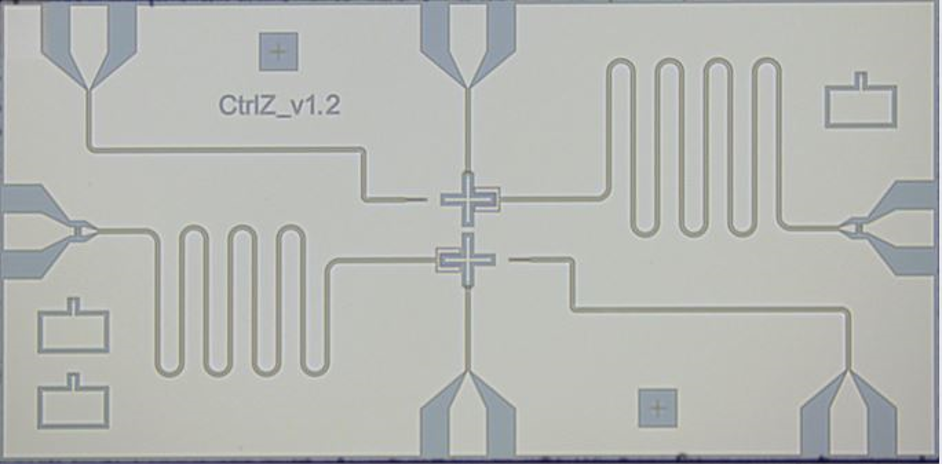
\includegraphics[width=12cm]{Chippic.png}
            \caption{作製したサンプル}
        \end{center}
    \end{figure}
    本サンプルは厚さ450umのシリコン基板に厚さ50nmのNbをスパッタした縦2.5$\times$横5mmのチップに加工を施し作製した。
    図の中央にある2つの十字はTunableなTransmon型量子ビットである。この形のTransmonは別名Xmon\cite{barends2013coherent}とも呼ばれ、
    周囲のコンポーネントとの配線のしやすさ、コヒーレンス時間の長さから電荷量子ビットベースの量子コンピュータで主流の形状である。\footnote{他にも繋げられる配線数を重視したTransmonとして多脚のStarmon,円形のConcentric Qubitなどのデザインも研究されている}
    量子ビット同士はキャパシティブに結合されている。量子ビットにつながる配線のうち、蛇行している配線はCPW(後述)である。図の垂直方向にXmonに向かって配線されているラインは量子ビットに磁束バイアスを与えるためのバイアスラインである。この図では見えづらいが、量子ビットのバイアスライン側にはAl-AlOx-AlからなるSQUIDがついており、バイアスラインから流す直流電流でSQUID内の磁束を調整する。
    チップ左上および右下から伸びている配線は1qubit回転ゲートのためのマイクロ波をXmonに送り込むコントロールラインとなっている。
    その他左下、右上に配置された凸型の素子は各々の量子ビットのテスト用ジャンクションであり、バイアスラインのポートとコントロールラインのポート間にあるのはアライメントマークである。
\subsubsection{CPW}
CPW (Coplanar Waveguide,コプレーナ共振器) は図のような構造をした共振器である。
\begin{figure}[H]
    \begin{center}
        \includegraphics[width=10cm]{CPW_img.png}
        \caption{CPWの構造}
    \end{center}
\end{figure}
比誘電率$\epsilon_r$の基板上には接地導体を挟んで中央に導体の線路が通っている。
共振周波数は光速$c$,電磁波の伝播方向への長さ$l$,そして基板及び上部の空間の形状から決定される実効的な比誘電率$\epsilon_{eff}$を用いて
\begin{equation}
    \omega_{r}=\frac{c \pi}{l \sqrt{\epsilon_{e f f}}}
\end{equation}
で与えられる。\\ %ここで実効的な比誘電率の値には$\epsilon_{e f f}=6.33$を用いた。
共振器全体のQ値($Q_{load}$は、外部素子との結合に由来する外部Q値($Q_{ext}$)及び共振器そのものの品質による内部Q値$Q_{int}$の成分に分けられ
\begin{equation}
    \frac{1}{Q_{l}}=\frac{1}{Q_{int}}+\frac{1}{Q_{ext}}
\end{equation}
という関係がある。このうち内部Q値に関しては共振器の材質や作製プロセスに大きく依存するので、外部のコンポーネントとの結合をキャパシタンスなどで調整して全体のQ値を変えることになる。

\section{設計値・留意した点}
作製したサンプルの等価回路モデル図を図()に示す。
\begin{figure}[H]
    \begin{center}
        \includegraphics[width=14cm]{Circdiagram.png}
        \caption{作製したサンプルの等価回路図}
    \end{center}
\end{figure}
図()の各種コンポーネントの周波数、キャパシタンス等の値の決定にあたっては、状態操作及び読み出しを適切に行うために、いくつかの制約が存在する。
\subsection{共振器の設計}
まず共振器については、我々の研究室が所有するローパスフィルタが$4 \sim 8$GHz,$8 \sim 12$GHzのレンジにあるため
4または8GHzの上下にまたがる周波数は避けるべきである。また共振器の周波数が低すぎると()式から共振器長を延長しなければならず
チップの限られたスペースを圧迫するため好ましくない。分散読み出しの条件$(\Delta = |\omega_r − \omega_q|\gg g)$を達成するために共振器と量子ビットの周波数を1GHz程離す必要があり、結合定数$g_{01}$も大きくて100MHz台に抑制される。
最後に、共振器からの光子放出レート$\kappa$について、これが弱結合領域($\kappa<g_{01},\Gamma_1$)の範囲に来るように設定した。この領域では状態読み出しが遅くなるものの
量子ビットのエネルギー緩和を低くとどめられる。
これらのことを考慮した上でシミュレーションを通じて共振器に関係するパラメータを以下のように定めた。
値の見積もりに際しては
\begin{table}[H]
    \begin{center}
    \begin{tabular}{c}
        \begin{minipage}{0.45\hsize}
            \begin{center}
                \begin{tabular}{|c|c|}
                    \hline
                    & [GHz] \\
                    \hline
                    \hline
                        共振器1の周波数$f_{r1}$ & 6.5 \\
                    \hline
                        共振器1の光子放出レート$\kappa_1$ & 2.3 [MHz]
                    \hline
                        共振器2の周波数$f_{r2}$ & 7.4 \\
                    \hline
                        共振器2の光子放出レート$\kappa_2$ & 1.6 [MHz]
                    \hline
                        量子ビット1と共振器1の結合定数$g^{01}$ & 0.068\\
                    \hline
                        量子ビット2と共振器2の結合定数$g^{01}$ & 0.073 \\
                    \hline
                \end{tabular}
            \end{center}
        \end{minipage}

        \begin{minipage}{0.4\hsize}
            \begin{center}
              \begin{tabular}{|c|c|}
                \hline
                \hline
                 & [fF]\\ 
                \hline 
                \hline
                $f_{r1}$ &  6.8\\
                $f_{r2}$ &  6.0\\
                $C_{in,1}$ &  8.0\\
                $C_{in,2}$ &  7.1\\
                \hline
              \end{tabular}
            \end{center}
          \end{minipage}
          \caption{共振器関係のパラメータ}
        \end{tabular}
    \end{center}
\end{table}
\subsection{量子ビットの設計}
量子ビットの固有周波数$\omega_q$は,$E_J,E_C$を用いて以下のように表される。
\begin{equation}
    \omega_q = \sqrt{8E_JE_C}-E_C \\
\end{equation}
このとき
\begin{equation}
    \begin{aligned}
        E_C &= \frac{e^2}{2C_{\Sigma}}\\
        C_{\Sigma} & = C_B+C_g+C_J\\
        E_J &= E_{J,max}|\cos(\pi \Phi/\Phi_0)| \\
        E_{J,max} &= \frac{I_C}{2e} \\
        I_C &= J_{C}A\\
        J_{C}&=\frac{\pi \Delta(T)}{2 e R_{n} A} \tanh \left(\frac{\Delta(T)}{2 k_{B} T}\right)
    \end{aligned}
\end{equation}
量子ビット間の結合定数$J$は結合部のキャパシタンス$C_c$を用いて
\begin{equation}
    J=C_{c} \approx \frac{1}{2} \frac{C_{c}}{\sqrt{C_{\Sigma}^{(1)} C_{\Sigma}^{(2)}}} \sqrt{\omega_{\mathrm{q}}^{(1)} \omega_{\mathrm{q}}^{(2)}}
\end{equation}
として見積もった。\\
ジョセフソン接合のキャパシタンス$C_J$については自分で設計できる量ではないので2~3fF程度として計算した。
2量子ビット直接結合系の場合、量子ビット同士の周波数が近すぎると一方のビットに送られたマイクロ波で他方のビットが状態操作される可能性があるため\footnote{原理の章での説明を省いたが、この作用を積極的に利用する、CR(Cross-Resonance)ゲートと呼ばれる2量子ビットゲートも存在する。CRゲートは特定のゲート時間だけ一方の量子ビットを他方の量子ビットの共振周波数のマイクロ波で駆動することにより、CNOTのユニタリ演算を実現できる。}
そのため、設計の上では量子ビットの周波数を800MHzほど離調している。量子ビット同士の結合定数$J$は強くなるほど式()よりゲート時間が短くなるが
状態操作を行わない状態での量子ビット間のエネルギー交換も行われやすくなるため大きくても20MHz台に設計する。\\
\begin{table}[H]
    \begin{center}
    \begin{tabular}{c}
        \begin{minipage}{0.45\hsize}
            \begin{center}
                \caption{量子ビット1,2の周波数単位のパラメータ}
                \begin{tabular}{|c|c|}
                    \hline
                    & [GHz] \\
                    \hline
                    \hline
                        量子ビット1の周波数$\omega_{q1}$ & 5.78 \\
                    \hline
                        〃非調和性$\alpha_{1}$ & -0.304\\
                    \hline
                        量子ビット2の周波数$\omega_{q2}$ & 6.61 \\
                    \hline
                        〃非調和性$\alpha_{1}$ & -0.298 \\
                    \hline
                        $E_{C1}$ & 0.27 \\
                    \hline
                        $E_{J1}$ & 17 \\
                    \hline
                        $E_{C2}$ & 0.27 \\
                    \hline
                        $E_{J2}$ & 22 \\
                    \hline
                        結合定数$J$ & 0.015\\
                    \hline
                \end{tabular}
            \end{center}
        \end{minipage}

        \begin{minipage}{0.4\hsize}
            \begin{center}
              \caption{キャパシタンスのシミュレート結果}
              \begin{tabular}{|c|c|}
                \hline
                \hline
                 & [fF]\\ 
                \hline 
                \hline
                $C_{B1}$ & 71.745 \\
                $C_{B2}$ & 71.745\\
                $C_{g1}$ &  6.8\\
                $C_{g2}$ &  6.0\\
                \hline
              \end{tabular}
            \end{center}
          \end{minipage}
        \end{tabular}
    \end{center}
\end{table}
\section{電磁界シミュレーション}共振器の周波数、各種キャパシタンスはCAD上で図面を設計し、AWR Micrwave officeというソフトウェアを用いてシミュレートした。
Microwave officeでは2次元図面に厚みを設定して誘電体と金属の層に対する設定を行うことで3次元に近い状況でのシミュレーションを行う。
また、超伝導体については電気抵抗がほぼない導体(電気伝導度=$10^{200}$)に近似した。\\
\begin{figure}[H]
    \begin{center}
        \includegraphics[width=14cm]{keisokutyuu.PNG}
        \caption{Microwave officeに取り込んだサンプル図面。共振器2の周波数特性をシミュレート中}
    \end{center}
\end{figure}
\begin{figure}[H]
    \begin{center}
        \begin{tabular}{c}
            \begin{minipage}{0.5\hsize}
                \begin{center}
                    \includegraphics[width=6cm]{Interdigitalcap.PNG}
                \end{center}
                %\captionsetup{labelformat=empty,labelsep=none}
                \caption{Interdigital capacitor}
            \end{minipage}
            
            \begin{minipage}{0.5\hsize}
                \begin{center}
                    \includegraphics[width=6cm]{keisokutyuu_bias.PNG}
                \end{center}
                %\captionsetup{labelformat=empty,labelsep=none}
                \caption{量子ビット付近拡大}
            \end{minipage}
        \end{tabular}
    \end{center}
\end{figure}
読み出しポート近くを拡大すると、Interdigital capacitorが配置されており、この形状の微調整により$C_in$の大きさを調節した。
またバイアスライン付近は図()のようになっているが、Microwave officeはインダクタンスを含めたシミュレーションはできないのでこの時点でSQUIDループは解析に加えていない。
まず共振器については図()のようにポートを配置し、ポート1からグラウンドポート-1に向けて送信するマイクロ波の反射係数S11を見ることで周波数特性を解析した。
量子ビット1,2にそれぞれ接続された共振器R1,R2の周波数特性は図()のとおりである。最終的にはこの曲線をResonator-tools \url{https://github.com/sebastianprobst/resonator_tools}を用いてfittingし
$Q_{in},Q_{out},\kappa$を求めた。
\begin{figure}[H]
    \begin{center}
        \includegraphics[width=10cm]{R1R2freq.png}
        \caption{共振器1,2の共振周波数}
    \end{center}
\end{figure}
また、ポート間のアドミタンス$Y$の周波数特性を見ることでコンポーネント間のキャパシタンスを見積もることもできる。インピーダンスを$Z$とすると
\begin{equation}
\begin{aligned}
    Z = R + j\omega L + \frac{1}{j\omega C} \\
    Y = 1/Z
\end{aligned}
\end{equation}
であり、超伝導体では$R \to 0$となる。さらに$\omega$が小さい領域では$L$を含む項の寄与は無視できるため
\begin{equation}
        Y \sim j\omega C
\end{equation}
と表現される。アドミタンスの虚部を$f$に対してプロットすると傾き$2\pi C$が得られ、ここからCの値が得られる。
(Im[Y]を測る周波数領域は$f=0 \sim 1.0$GHzまでとした。)
\section{作製手順}
チップの作製にあたっては理化学研究所内クリーンルームにてパッケージングを除く全作業を行った。このうちの大まかな工程について述べる。
\subsubsection{1.Photolithography}
デザインにおけるジョセフソン接合以外の部分(共振器,量子ビット本体)をチップ上にパターニングする工程。
ここでは2×2cmのチップに2.5×5mmのデザインを8×4個配置したパターンを一遍に描画した。
レジストとしてZEP520A-7をスピンコーターを用いて塗布し、マスクレスUV露光装置を用いてUVを照射。
現像後、CF4ガスによるエッチングを施し、残留レジストを剥離液で洗い流す。
\subsubsection{2.EBL}
続いて電子ビーム描画装置によりジョセフソン接合部分のパターンを描画した。
先ほどのUVを照射するPhotolithographyと比較してビーム径が小さいので、より精緻なデザインを描画できる。
2層のレジストZEP520A-7, Copolymerを塗布しホットプレートで焼き固め、ビーム照射後に上層のZEPのみを現像した。
その後IPA(イソプロピルアルコール)と超純水93:7溶液でZEPに穴が空いた箇所のCopolymerを現像した。
ここまでの作業によりSQUID付近には図()に示す、ジョセフソン接合を蒸着するための空洞が形成される。
\subsubsection{3.PLASSYS}
\begin{figure}[H]
    \begin{center}
        \includegraphics[width=16cm]{PLASSYS_stage0.png}
        \caption{EBL終了後のレジストによる空洞}
    \end{center}
\end{figure}
\begin{figure}[H]
    \begin{center}
        \includegraphics[width=16cm]{PLASSYS_stage1.png}
        \caption{2角度蒸着法:一回目のアルミ蒸着後}
    \end{center}
\end{figure}
\begin{figure}[H]
    \begin{center}
        \includegraphics[width=16cm]{PLASSYS_stage2.png}
        \caption{アルミの酸化被膜形成}
    \end{center}
\end{figure}
\begin{figure}[H]
    \begin{center}
        \includegraphics[width=8cm]{JJ_img_zoomup.png}
        \caption{ジョセフソン接合,重なり部分}
    \end{center}
\end{figure}
ジョセフソン接合はAl-AlOx-Alの重なりを作るために2角度蒸着法という工程によって形成される。
最初に少し角度$\theta$をつけた状態で一層目のアルミが蒸着され、10分程O2ガスによって酸化されたのち
二層目のアルミが先ほどとは逆向きに同じ角度で蒸着される。一層目の酸化被膜がジョセフソン接合の薄膜障壁の役割を果たし、
この被膜と2層目のアルミの重なり面積によりここを通るジョセフソン電流の臨界電流値が決定される。
重なり面積$S$は図中に示すパラメータを用いて
\begin{equation}
    S = (2y \tan \theta -g)R
\end{equation}
と求められ、電流密度Jが既知であれば式(),()により$I_{J,max}$が求められる。
自身のサンプルで設計に用いた値を表()に示す。
\begin{table}[H]
    \caption{ジョセフソン接合作製時のパラメータ}
    \begin{center}
    \begin{tabular}{|c|c|}
    \hline
     & [nm]\\
    \hline
    \hline
    x & 300\\
    \hline
    y & 600\\
    \hline
    R & Q1側:250, Q2側:320\\
    \hline
    w & 350 \\
    \hline
    g & 295 \\
    \hline
    \end{tabular}
\end{center}
\end{table}
蒸着後、接合部ではない箇所のアルミを剥離液で剥がし、SEM(走査電子顕微鏡)によりジャンクションが形成されていることを確認した。
SEMによるジャンクション付近の撮影の結果を図()に示す。
\begin{figure}[H]
    \begin{center}
        \begin{tabular}{c}
            \begin{minipage}{0.5\hsize}
                \begin{center}
                    \includegraphics[width=6cm]{Ino_test_up.jpg}
                \end{center}
                %\captionsetup{labelformat=empty,labelsep=none}
                \caption{2角度蒸着法で形成されたジョセフソン接合}
            \end{minipage}
            
            \begin{minipage}{0.5\hsize}
                \begin{center}
                    \includegraphics[width=6cm]{Ino_test_upL.jpg}
                \end{center}
                %\captionsetup{labelformat=empty,labelsep=none}
                \caption{接合部の拡大図}
            \end{minipage}
        \end{tabular}
    \end{center}
\end{figure}
\subsubsection{4.Dicing}
UVレジストを塗布・焼き固めたのち、チップを2.5×5mmに切り出す。アセトンとIPAでレジスト剥離、洗浄を行いチップが完成する。
\subsection{パッケージング}
完成したサンプルは専用のサンプルホルダー(図())に装着される。
\begin{figure}[H]
    \begin{center}
        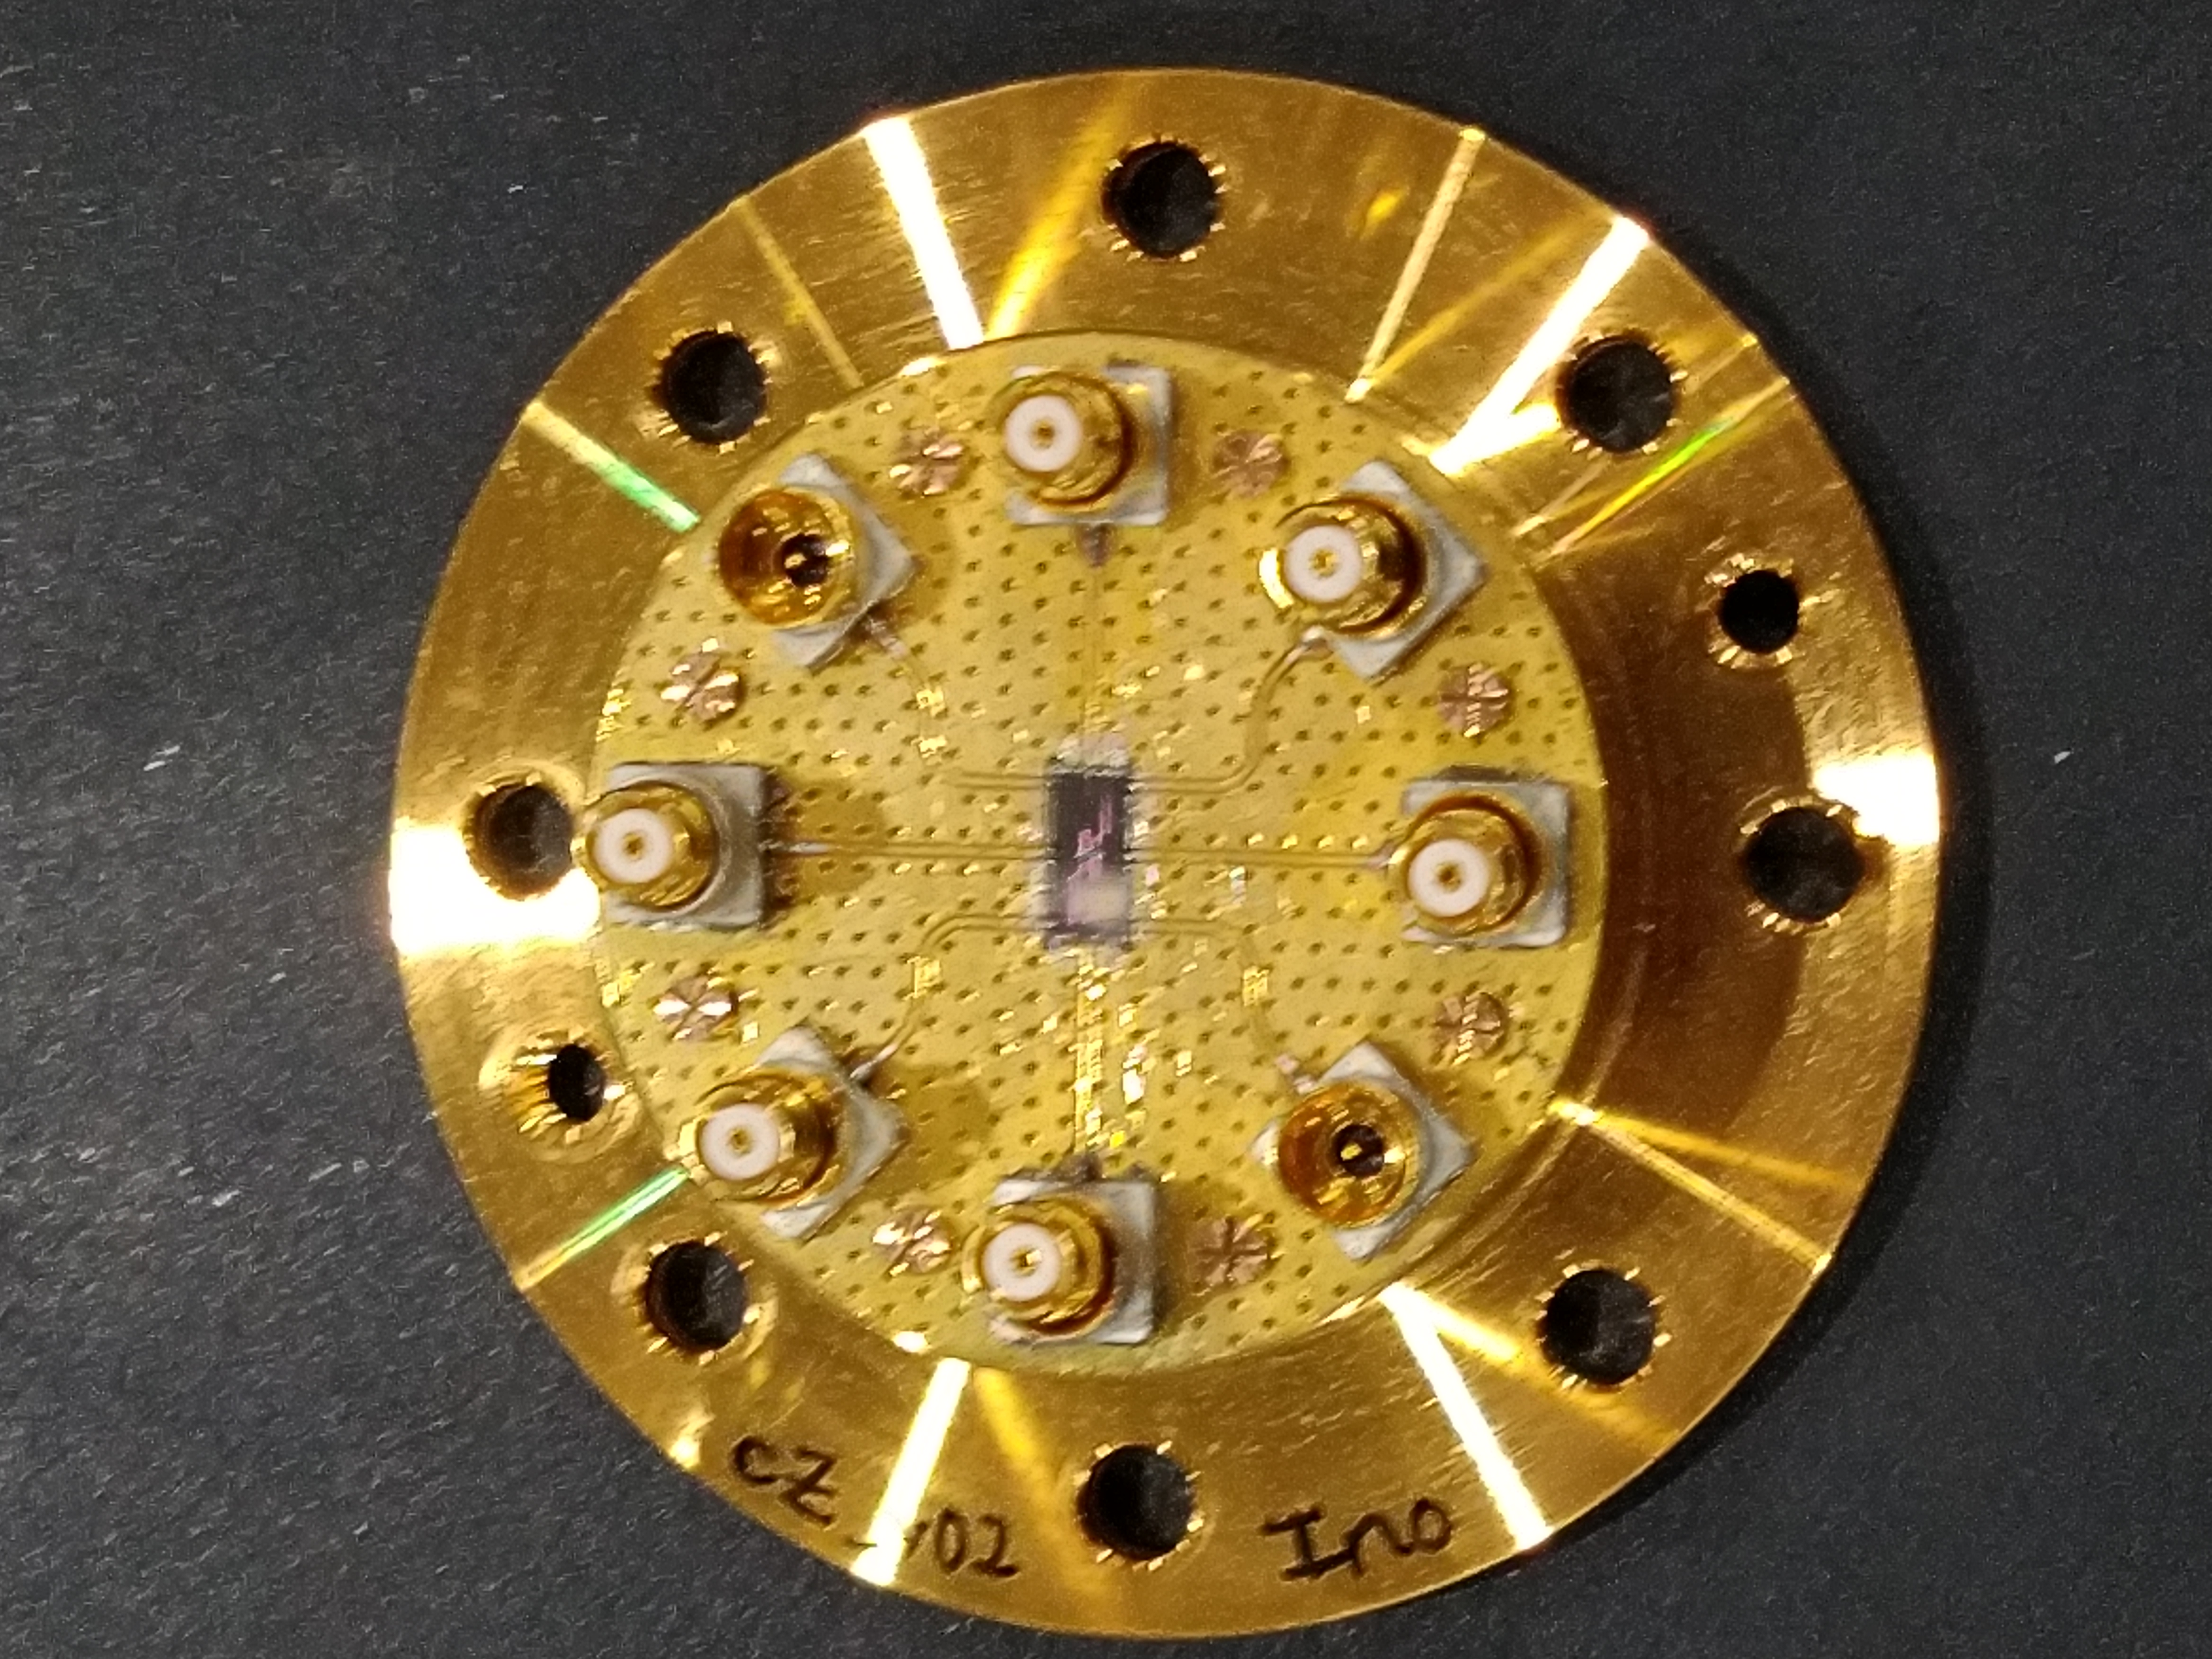
\includegraphics[width=7cm,angle=-90]{sample_from_above.jpg}
        \caption{サンプルホルダーに装着されたチップ}
    \end{center}
\end{figure}
サンプルホルダー上面はPCB(Printed Circuit Board,プリント基板)となっており
チップの固定ならびに接続されたSMAコネクタ経由で送られてくる信号をチップ上のポートに伝送する役割を担う。
\begin{figure}[H]
    \begin{center}
        \begin{tabular}{c}
            \begin{minipage}{0.5\hsize}
                \begin{center}
                    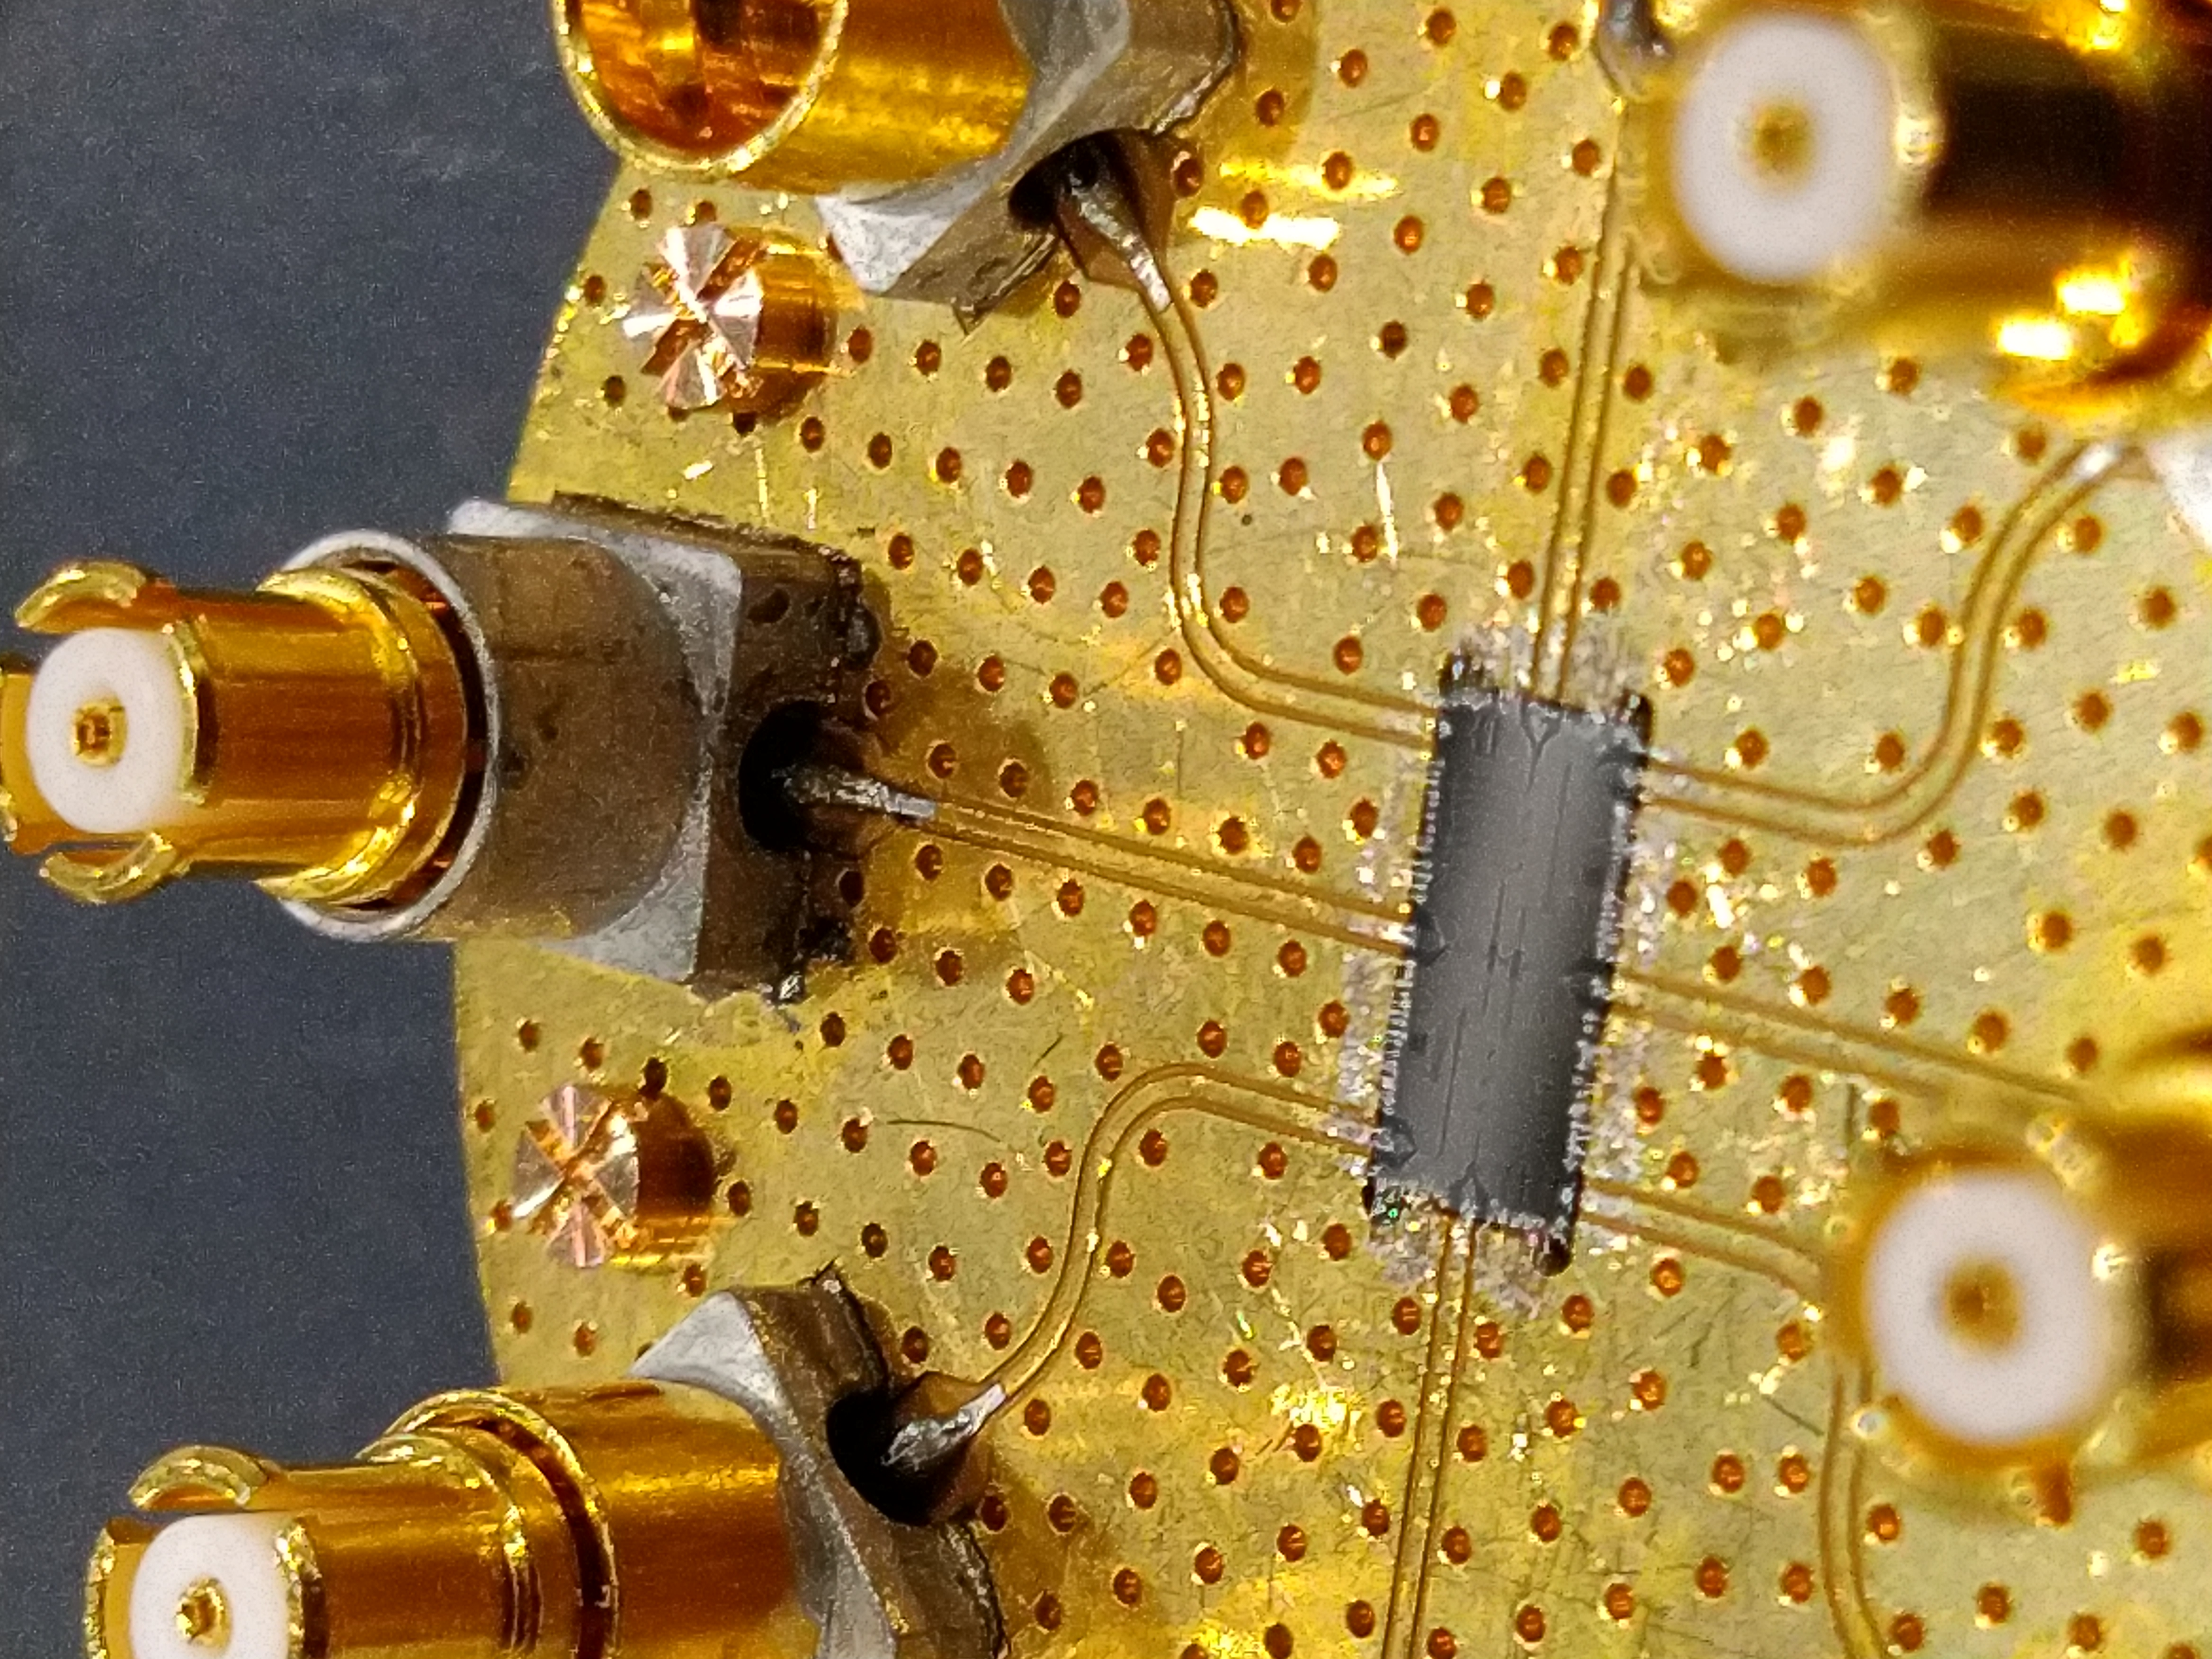
\includegraphics[width=6cm,angle=-90]{zoomup_SMA_PCB.jpg}
                \end{center}
                %\captionsetup{labelformat=empty,labelsep=none}
                \caption{サンプルを装着したPCB(拡大)}
            \end{minipage}
            
            \begin{minipage}{0.5\hsize}
                \begin{center}
                    \includegraphics[width=7cm]{Kansei1.jpg}
                \end{center}
                %\captionsetup{labelformat=empty,labelsep=none}
                \caption{Bondingされたチップ}
            \end{minipage}
        \end{tabular}
    \end{center}
\end{figure}
サンプルをホルダーに装着しただけではポートに信号が流れないため、チップのポートとPCBのポート、及びチップのGroundとPCBのGroundはアルミニウム細線により
複数箇所で接続(Bonding)される。
Bonding終了後はスペーサーと呼ばれるカバーを装着し希釈冷凍機に導入される。


